\chapter{Background}

\label{Chapter1} 

\begin{comment}
-------------------------------------------------
%								Chapter layout
2. Background
	a. Leap Motion (v2)
		i. Java API and Native Libraries
		ii. Limitations of Sensor and Documentation
	b. JavaFx
		i. Java vs FXML
		ii. SceneBuilder
		iii. Jfoenix
-------------------------------------------------
\end{comment}



%------------------------------------------------
%	SECTION 1 Leap Motion (v2)
%------------------------------------------------
\section{Leap Motion}
Leap Motion controller, developed by Leap Motion Inc, US based company located in San Francisco, is a small infrared-enabled sensor that can be attached to one’s computer via a USB cable. It comes with its own software that allows it to detect a user’s hand movements in 3D space without any physical touch. It also can detect simple tools being held in the hand such as a pencil. The Leap Motion controller accomplishes this via two cameras and three embedded infrared LEDs which are able to track infrared light with wavelength outside that of the visible light spectrum. The sensor is able to detect motion in a wide space of around 8 cubic feet of area around it. This interaction area can be visualized as an inverted pyramid emanating from the Leap Motion sensor with a height, width and length of 2 cubic feet; as shown in Figure \ref{fig:LeapInteractionArea}.
\begin{figure}[th]
\centering
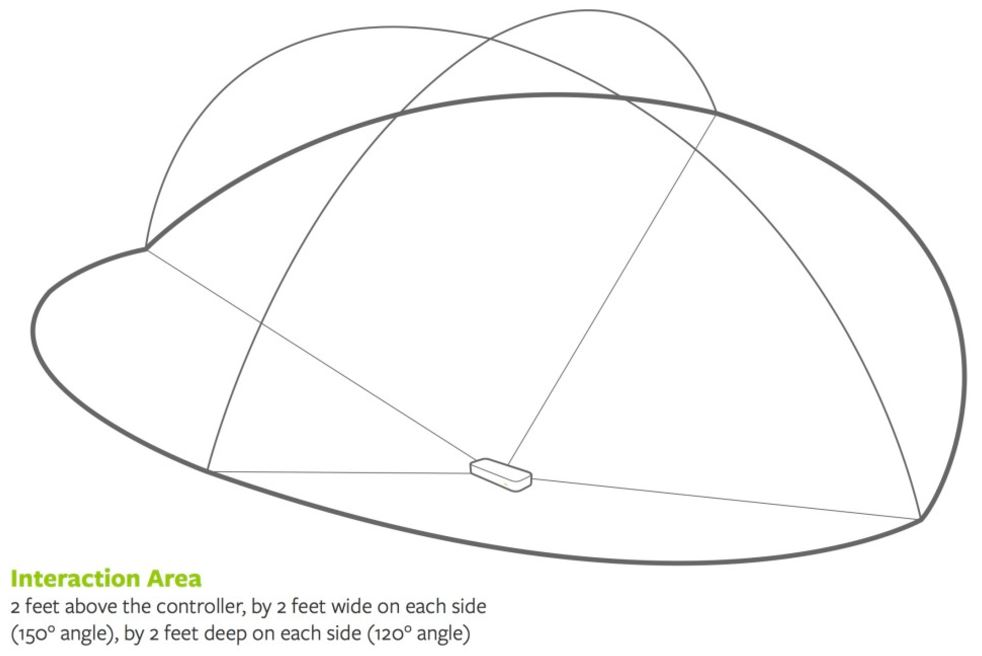
\includegraphics[scale=0.35]{Figures/LeapInteractionArea.JPG}
\caption[Leap Motion interaction area]{The area of user interaction for the Leap Motion Device.}
\label{fig:LeapInteractionArea}
\end{figure}

	
%----------------------------------- Leap Motion Java API
\subsection{Leap SDK v2 Java API}
%discuss about lm native libraries. 
When the Leap Motion software is installed on one's computer, it does not include the libraries needed in order to develop applications utilizing the controller. In order to do that, the appropriate SDK version of the software must be downloaded from Leap Motion's website. The Java SDK version includes a JAR file and two native library files. The JAR file contains the Leap Motion API class definitions and the native libraries are OS platform specific files which allow a program using the Leap Motion API to communicate to the underlying service (Windows) or daemon (Linux or Mac) which is running the Leap Controller. Setting up a Java project requires that the distributed JAR file be set to the project's classpath. When running such a project, the JVM's library path parameter must be set to the location of the native libraries. A further discussion into the technicalities of setting up a Leap Motion Project in the Intellij IDE is carried out in Appendix A.


%api/data model general discussion
In this paragraph the data model that Leap Motion uses to represent the raw data received from device's cameras will be discussed. This data model consists of Frame objects that are continuously taken at a set rate of 60fps. These Frame objects contain all of the tracked data the Leap Motion sensor recorded in its field of view at a certain instance in time. The objects that the device keeps track include the two hands, their fingers and arm positions as estimated by normal human proportions. There are corresponding Java classes to represent these objects, such as the Hand, Finger, and Arm class. There is also a Bone class to represent specific types of bones in a hand. The Leap Motion Hand model is able to provide information about the identity, position, direction, rotation angles and other characteristics of the detected hand that it represents. This Hand model also contains methods which allow one to access other model objects contained within it; for example the fingers or the arm. Leap Motion software uses an internal hand model of the human hand to assist it in making predictions about the positions of certain parts of the hand even if they are not visible to the infrared cameras and thus not able to be calculated from the tracking data. The API also provides a Vector class that allows for useful math operations involving vectors such as finding the distance, dot product or cross product between them. 

%specific example
To understand the Leap Motion Java API more clearly, a very simple example will be presented that shows how the Frame data can be received from the device. Firstly, it is assumed that the project has been set up with the correct classpath for the Leap Motion Java SDK JAR file and run time parameters pointing to the appropriate native libraries. Figure \ref{fig:leapMotionSample} shows the basic set-up required to receive data from the controller using the Leap Java API. 

\begin{figure}[th]
\centering
\begin{lstlisting}
import com.leapmotion.leap.*;

//Listener class which handles various events for the Controller
class SampleListener extends Listener {
    //method to handle the event of a Frame received from Controller
    public void onFrame(Controller controller) {
        // Get the most recent frame and report some basic information
        Frame frame = controller.frame();
        System.out.println("Frame id: " + frame.id() + ", hands: " + frame.hands().count()
    }
}

class Sample {
    public static void main(String[] args) {
        // Create leap motion controller instance
        Controller controller = new Controller();

        // Have the sample listener receive events from the controller
        controller.addListener(new SampleListener(););

        // Remove the sample listener when done
        controller.removeListener(listener);
    }
}
\end{lstlisting}
\caption[Leap Motion Sample]{This code sample shows how to connect to and receive data from the Leap Motion controller device.}
\label{fig:leapMotionSample}
\end{figure}





%------------------------------------------------
%	SECTION 2 JavaFX
%------------------------------------------------
\section{JavaFx}
JavaFX is a framework provided by Oracle Corporation that is intended to replace the Swing framework as the standard GUI library for developing desktop applications that can be run on any platform that supports Java. Since the JavaFX 2.0 release, JavaFX application can be written in pure Java code. Before that release, applications written using JavaFX libraries had to be written in JavaFX Script, a scripting language designed and used specifically for the purpose of creating GUI applications with JavaFX. This project uses the latest version of this framework, JavaFX 8, which also added support for 3D graphics and sensor support. 


%----------------------------------- Java vs FXML
\subsection{Java vs FXML}
When writing a JavaFX application, there are two very different approaches that can be used to create the actual user interface (UI) for the application. These are pure Java code and FXML. A brief introduction both of these approaches will be given below. 

The pure Java approach constructs the JavaFX application scene graph procedurally through code. Below is a simple “Hello World” program that shows a quick example of this approach in action.
\begin{figure}[th]
\centering
\begin{lstlisting}
public class HelloWorld extends Application {
public static void main(String[] args) {
	launch(args);
}

@Override
public void start(Stage primaryStage) {
	primaryStage.setTitle("Hello World!");
	Button btn = new Button();
	btn.setText("Say 'Hello World'");
	btn.setOnAction(new EventHandler<ActionEvent>() {
		@Override
		public void handle(ActionEvent event) {
			System.out.println("Hello World!");
		}
	});
	
	StackPane root = new StackPane();
	root.getChildren().add(btn);
	primaryStage.setScene(new Scene(root, 300, 250));
	primaryStage.show();
}
}
\end{lstlisting}
\caption[JavaFX HelloWorld]{A simple hello world program using JavaFX written using just Java code.}
\label{fig:helloWorldJavaFX1}
\end{figure}
This small snippet of code contains the overall structure and all of the basic components of a JavaFX application. The first point to note is that the main class which will run the JavaFX application must extend from the abstract base class called javafx.application.Application and implement is abstract start() method. The start() method serves as the main entry point for all JavaFX applications. In the application’s main() method, which is common to all Java applications, a call must be made to the launch() method which is a method defined in the base Application JavaFX class that actually launches the application in doing so makes a call to the start() method. 

The start() method receives a parameter of type Stage which serves as the primary Stage object for the application. Stage is the top-level user interface container object used by JavaFX to house the whole application. In colloquial terms it can be considered to be the “window” object of the whole application. The Stage object is has a setScene() method which requires a Scene object to be passed in. Scene class is the container of current content being displayed by the application. An application can have multiple scenes which display different pages of the the application. In JavaFX, the actual UI components, such as the StackPane layout Node shown in the simple HelloWorld example above, must be added to the Scene object in order for them to be displayed. This relationship between the Stage, Scene and “root” Node components of a JavaFX application is depicted in Figure \ref{fig:stageSceneRoot}.
\begin{figure}[th]
\centering
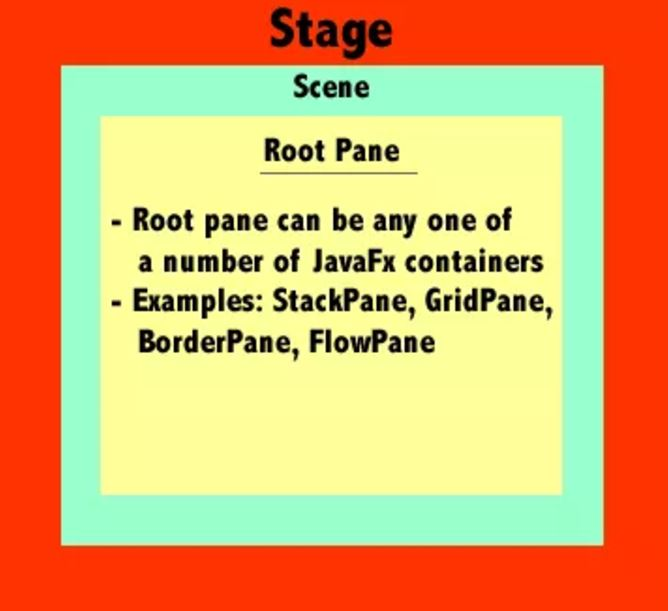
\includegraphics[scale=0.5]{Figures/stageSceneRoot.JPG}
\caption[UI Layout]{The layout components of every JavaFX application.}
\label{fig:stageSceneRoot}
\end{figure}

The UI components all extend from a parent Node class. One of the improvements that JavaFX brought in regards to its predecessor Swing, is that it represents the entire content of the scene as a tree. More specifically, all of the nodes displayed in a Scene container object must extend from a root level node and be part of the hierarchical scene graph of nodes. Figure \ref{fig:javafxSceneGraph}  displays an example of the JavaFX scene graph.
\begin{figure}[th]
\centering
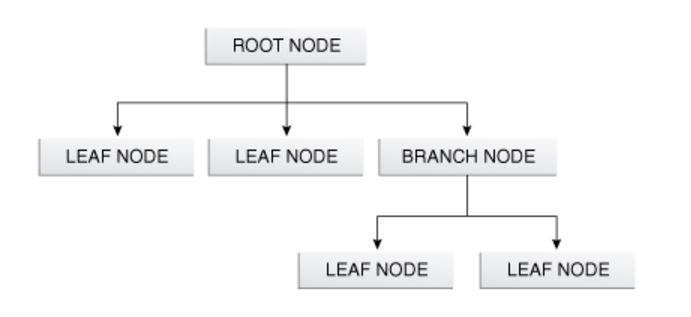
\includegraphics[scale=0.5]{Figures/javafx_scenegraph.JPG}
\caption[JavaFX Scene Graph]{The Scene Graph architectural model for UI components in JavaFX applications.}
\label{fig:javafxSceneGraph}
\end{figure}

Now that the pure Java code approach of writing JavaFX applications has been introduced, let us discuss the other approach to writing JavaFX applications; FXML. FXML is an XML-based language created by Oracle Corporation for the purpose of making it easier to define the UI of a JavaFX application. While the pure Java code approach is a much more imperative and procedural way to write JavaFX applications, FXML is a more declarative way. It resembles HTML and can also reference a controller java class which can access and modify the UI elements defined in the FXML file. Figure \ref{fig:simpleFXML} shows a very simple FXML file that creates a VBox layout and adds a button to it. This FXML file also has a Java controller class attached to it which is called MyController.java and shown in Figure \ref{fig:simpleController}

\begin{figure}[th]
\centering
\begin{lstlisting}
<?xml version="1.0" encoding="UTF-8"?>
<?language JavaScript?>
<?import javafx.scene.control.*?>
<?import javafx.scene.layout.*?>

<VBox fx:id="myView" layoutX="10.0" layoutY="10.0" xmlns:fx="http://javafx.com/fxml/1" xmlns="http://javafx.com/javafx/2.2" fx:controller="MyController">
  <children>
    <Button fx:id="okBtn" alignment="CENTER_RIGHT" contentDisplay="CENTER" mnemonicParsing="false" onAction="#printHelloWorld" text="Say Hello World" textAlignment="CENTER" />
  </children>
</VBox>
\end{lstlisting}
\caption[FXML example]{A FXML file defining a simple layout and referencing a controller java class.}
\label{fig:simpleFXML}
\end{figure}


\begin{figure}[th]
\centering
\begin{lstlisting}
public class MyController 
{
	@FXML
	private void initialize() 
	{
	// this method runs first after all the UI components have been loaded and bound.
	}
	
	@FXML
	private void printHelloWorld() 
	{
		System.out.println("hello world!");
	}
}
\end{lstlisting}
\caption[Controller for FXML]{A controller for the FXML file. The "FXML" annotation in is used to bind certain elements to Java objects in the class.}
\label{fig:simpleController}
\end{figure}

The result from both of these HelloWorld examples will be as showing in Figure \ref{fig:helloWorldResult}. The large difference between these two approaches makes it difficult to combine them effectively, but it is possible to use them in conjunction with each other. This project takes such an approach. For the UI construction of the user's hand model, the pure Java code approach was taken. However, for the interface of the application the table construction showing all of the collected data, the FXML approach was taken. 

\begin{figure}[th]
\centering
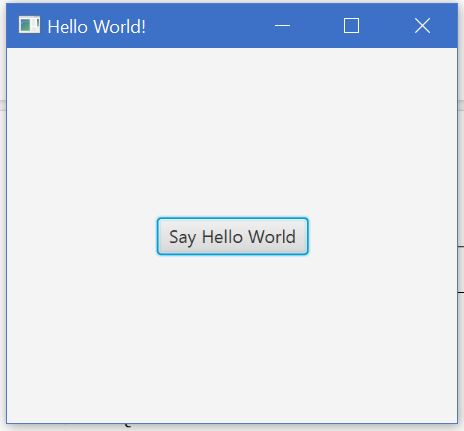
\includegraphics[scale=0.5]{Figures/helloWorldResult.JPG}
\caption[JavaFX Application Output]{The output of the simple HelloWorld application.}
\label{fig:helloWorldResult}
\end{figure}

One of the things that should be discussed is how communication can happen between different components of the application when FXML files are being used. There is a special class called FXMLLoader which is used to load FXML files and return the object graph of UI components these files contain. The FXMLLoader contains two \verb {load()} methods one of which is a static class method and the other is an instance method. The important difference between these two methods is that that instance \verb {load()} method can be used to gain access to the controller for the FXML class being loaded. Gaining access to the controller object for an FXML file in other other parts of an application is very important if one has to pass parameters into the view to change the interface. Figure \ref{fig:fxmlLoaderCode} this key difference between the two methods. 


\begin{figure}[th]
\centering
\begin{lstlisting}
// The approach uses the static "load" method. Not recommended
Parent root = FXMLLoader.load(getClass().getResource("fxml_example.fxml"));
 
//This approach allows one to access the controller. 
//create instance of FXMLLoader
FXMLLoader loader = new FXMLLoader(getClass().getResource("fxml_example.fxml"));
//get the controller
MyController controller = loader.<MyController>getController();
//initialize controller with custom parameters
controller.initData(data);
//object graph root handle
Parent root = (Parent) loader.load();
\end{lstlisting}
\caption[FXMLLoader]{Retrieving a reference to the controller object for a loaded FXML file.}
\label{fig:fxmlLoaderCode}
\end{figure}




%----------------------------------- SceneBuilder
\subsection{Scene Builder}
Scene Builder is a software that can be installed on one's computer to help design the UI and layout of a JavaFX application. It allows the user to drag and drop components from the library of available components to the central work area where they can be modified and their properties tweaked. This software is a free and open source tool that used to be developed by Oracle Corporation, but is now backed by Gluon. The easy to use drag and drop functionality of the Scene Builder allows for easy design and rapid iteration. The associated FXML code with UI created by Scene Builder can be incorporated into the JavaFX application. Using Scene Builder code bindings can also be placed on certain UI components to allow for them to execute specific logic that can be defined in the controller class of the FXML file. Figure \ref{fig:sceneBuilderWindow} shows the main layout of the Scene Builder application. There are four main panels of information that have been labeled appropriately in the figure. These are: the Library panel, which contains all of the UI components available for use; the Document panel, which shows the object graph hierarchy of the current scene being built; the Content panel, which shows the work area for user interaction; and finally the Inspector panel, which shows the various properties and layout parameters which can be modified for the currently selected UI component, as well as the various code bindings that can be placed on it. 

\begin{figure}[th]
\centering
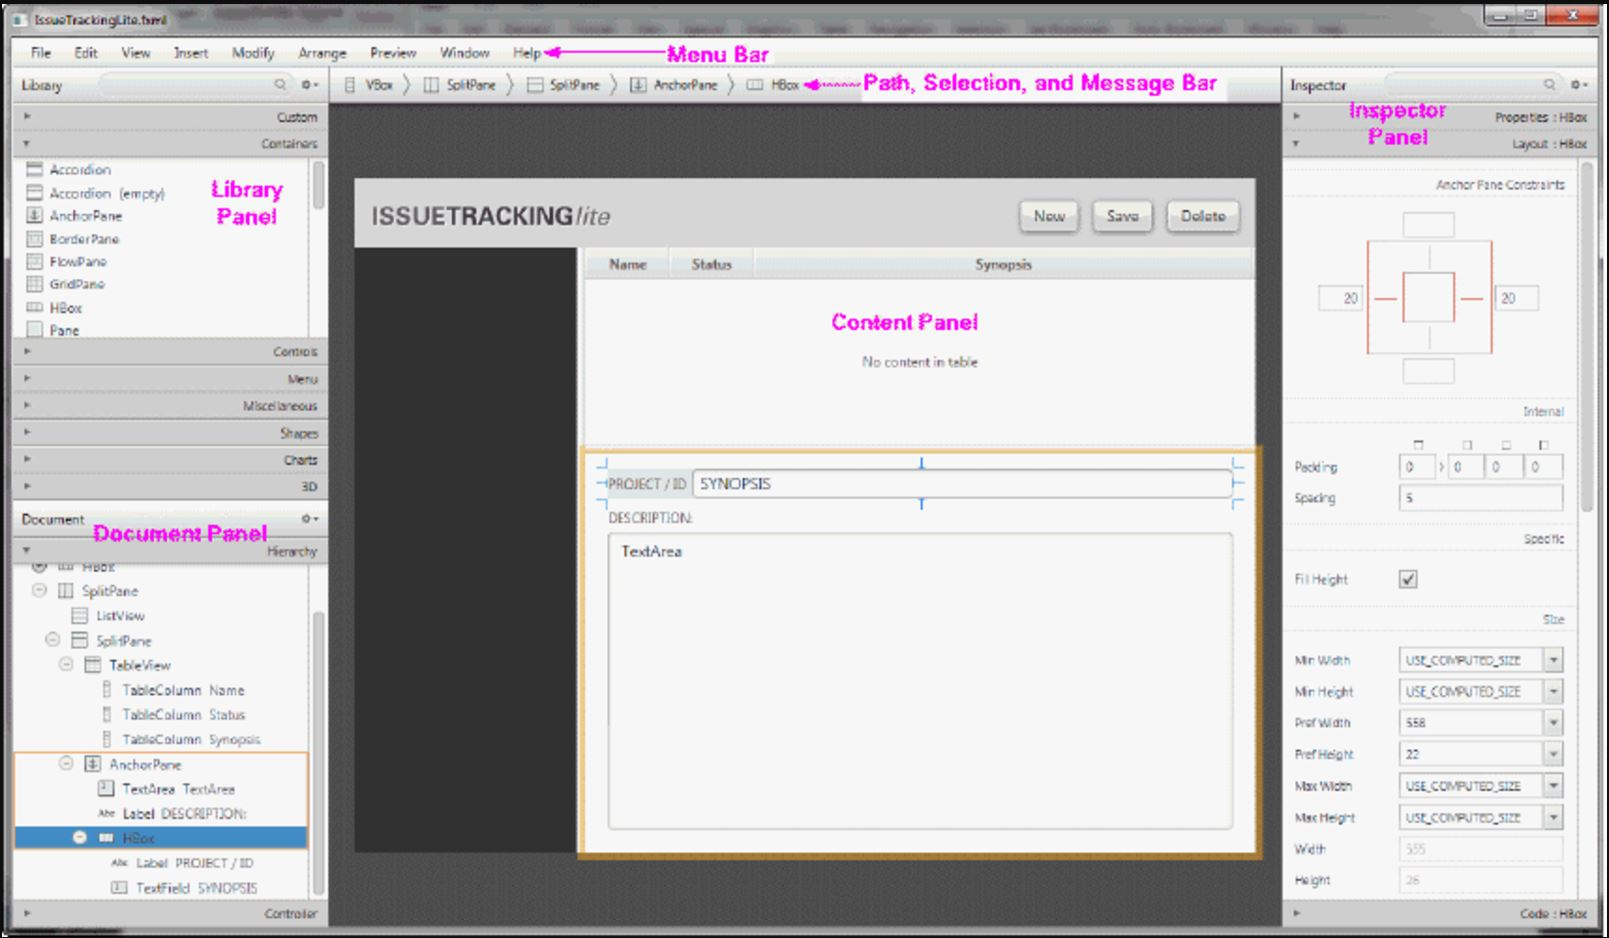
\includegraphics[scale=0.35]{Figures/sceneBuilderWindow.JPG}
\caption[Scene Builder]{This shows the different areas of interest in the Scene Builder software.}
\label{fig:sceneBuilderWindow}
\end{figure}




%----------------------------------- Jfoenix
\subsection{Jfoenix Library}
Jfoenix is a library that is used in this project. This is an open source Java library that implements Google Material Design for JavaFX components. This library can be included as a dependency via the Maven using the commands:  
\begin{lstlisting}
<dependency>
    <groupId>com.jfoenix</groupId>
    <artifactId>jfoenix</artifactId>
    <version>1.4.0</version>
</dependency>
\end{lstlisting}

Maven is a build automation tool that can also serve as a package manager that makes finding and installing dependencies simple. This library will be downloaded from Maven 2 Central Repository. To include this Jfoenix library within Scene Builder, one has to find where the JAR file for the Jfoenix library was downloaded. Then, going to Scene Builder, clicking on the gear icon in the Library panel will show a drop-down menu which has the option for "Import JAR/FXML File" as depicted in Figure \ref{fig:addLibrarySceneBuilder}. Selecting this option will allow for the Jfoenix JAR file to be specified and the custom components to be loaded into the Scene Builder. 
\begin{figure}[th]
\centering
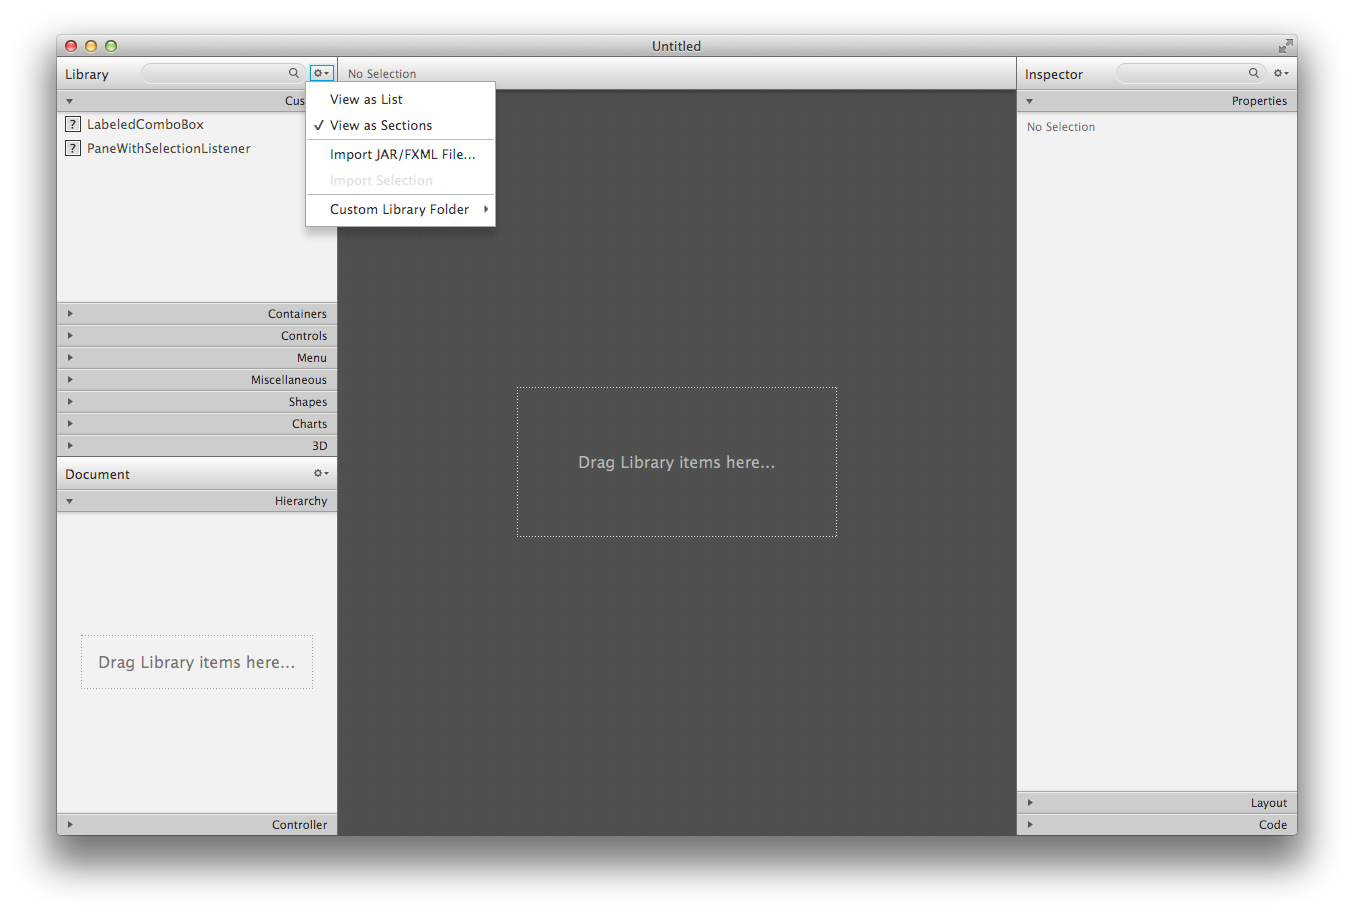
\includegraphics[scale=0.35]{Figures/addLibrarySceneBuilder.png}
\caption[External Libraries]{This is how to add a external library of custom components to the Scene Builder for UI prototyping.}
\label{fig:addLibrarySceneBuilder}
\end{figure}
